% Copyright 2004 by Till Tantau <tantau@users.sourceforge.net>.
%
% In principle, this file can be redistributed and/or modified under
% the terms of the GNU Public License, version 2.
%
% However, this file is supposed to be a template to be modified
% for your own needs. For this reason, if you use this file as a
% template and not specifically distribute it as part of a another
% package/program, I grant the extra permission to freely copy and
% modify this file as you see fit and even to delete this copyright
% notice. 

\documentclass{beamer}
\usepackage{menukeys}[os=win]
\usepackage{textcomp}
\usepackage{tcolorbox}
\usepackage{listings}
\lstset{
  basicstyle=\tiny\ttfamily,
}

% There are many different themes available for Beamer. A comprehensive
% list with examples is given here:
% http://deic.uab.es/~iblanes/beamer_gallery/index_by_theme.html
% You can uncomment the themes below if you would like to use a different
% one:
%\usetheme{AnnArbor}
%\usetheme{Antibes}
%\usetheme{Bergen}
%\usetheme{Berkeley}
%\usetheme{Berlin}
%\usetheme{Boadilla}
%\usetheme{boxes}
%\usetheme{CambridgeUS}
%\usetheme{Copenhagen}
%\usetheme{Darmstadt}
%\usetheme{default}
%\usetheme{Frankfurt}
%\usetheme{Goettingen}
%\usetheme{Hannover}
%\usetheme{Ilmenau}
\usetheme{JuanLesPins}
%\usetheme{Luebeck}
%\usetheme{Madrid}
%\usetheme{Malmoe}
%\usetheme{Marburg}
%\usetheme{Montpellier}
%\usetheme{PaloAlto}
%\usetheme{Pittsburgh}
%\usetheme{Rochester}
%\usetheme{Singapore}
%\usetheme{Szeged}
%\usetheme{Warsaw}
\setbeamerfont{block body}{size=\small}
\title{KF5004 - \texttt{DNS} Architecture and Caching Server}

% A subtitle is optional and this may be deleted
% \subtitle{(Using proximity detection)}

\author{Dr.~Neil~Eliot \& Dr.~Alun~Moon}
% - Give the names in the same order as the appear in the paper.
% - Use the \inst{?} command only if the authors have different
%   affiliation.

%\renewcommand\appendixname{Appendix}

\institute[Northumbria University] % (optional, but mostly needed)
{
  Department of Computer and Information Sciences\\
  University of Northumbria
  % \and
  % \inst{2}
  % Department of Theoretical Philosophy\\
  % University of Elsewhere
}
% - Use the \inst command only if there are several affiliations.
% - Keep it simple, no one is interested in your street address.

\date{Session 3}
% - Either use conference name or its abbreviation.
% - Not really informative to the audience, more for people (including
%   yourself) who are reading the slides online

\subject{Introduction}
% This is only inserted into the PDF information catalog. Can be left
% out. 

% If you have a file called "university-logo-filename.xxx", where xxx
% is a graphic format that can be processed by latex or pdflatex,
% resp., then you can add a logo as follows:

% \pgfdeclareimage[height=0.5cm]{university-logo}{university-logo-filename}
% \logo{\pgfuseimage{university-logo}}

% Delete this, if you do not want the table of contents to pop up at
% the beginning of each subsection:
% \AtBeginSubsection[]
% {
%   \begin{frame}<beamer>{Outline}
%     \tableofcontents[currentsection,currentsubsection]
%   \end{frame}
% }

% Let's get started

\begin{document}

\begin{frame}
  \titlepage
\end{frame}

\begin{frame}{Introduction}
  \tableofcontents
  % You might wish to add the option [pausesections]
\end{frame}

% Section and subsections will appear in the presentation overview
% and table of contents.

\section{Introduction to \texttt{DNS}}
\begin{frame}{What is \texttt{DNS}?}
  \begin{itemize}
    \item \texttt{DNS}
      \begin{itemize}
          \item \texttt{D}omain \texttt{N}ame \texttt{S}ervice
      \end{itemize}
    \item What does it do?   
      \begin{itemize}
        \item It is a translation database
        \item It maps \texttt{IP} addresses to domain names
        \item It maps domain names to \texttt{IP} addresses
          \begin{itemize}
            \item \texttt{rDNS}
          \end{itemize}
      \end{itemize} 
  \end{itemize}
  \begin{figure}
    \begin{center}
      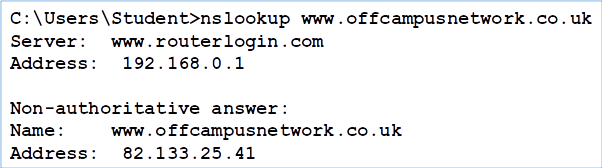
\includegraphics[width=0.8\linewidth]{nslookup.png}
    \end{center}
  \end{figure}
\end{frame}

\subsection{Installation}
\begin{frame}{Installing \texttt{DNS} on \texttt{Ubuntu Server}}
  \begin{itemize}
    \item The \texttt{DNS} server is in a package called \texttt{BIND9}
    \item You will also require the utilities that go with the server.
      \begin{itemize}
        \item \texttt{dnsutils}
      \end{itemize} 
    \item Installation of both these packages is performed using \texttt{apt-get}
  \end{itemize}
\end{frame}

\begin{frame}{Installing \texttt{DNS} on \texttt{Ubuntu Server}}
  \begin{itemize}
    \item \texttt{\$sudo apt-get install bind9 dnsutils}
  \end{itemize}
  \begin{figure}
    \begin{center}
      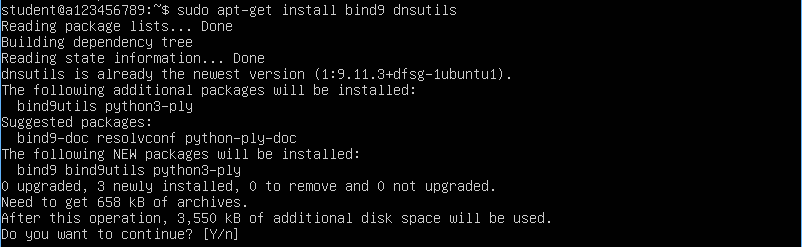
\includegraphics[width=0.9\linewidth]{bind9-1.png}
    \end{center}
  \end{figure}
  \begin{figure}
    \begin{center}
      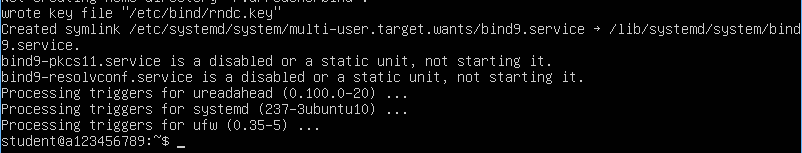
\includegraphics[width=0.9\linewidth]{bind9-2.png}
    \end{center}
  \end{figure}
\end{frame}

\begin{frame}{Installing \texttt{DNS} on \texttt{Ubuntu Server}}
  \begin{itemize}
    \item This gives a basic install of a fully functioning \texttt{DNS} server.
    \item This has very limited functionality and requires configuring before it is of any real use.
    \item You can check to see if it running using the \texttt{ps} command.
      \begin{itemize}
        \item \texttt{\$ps -ef | grep bind}
      \end{itemize}
    \end{itemize}
  \begin{figure}
    \begin{center}
      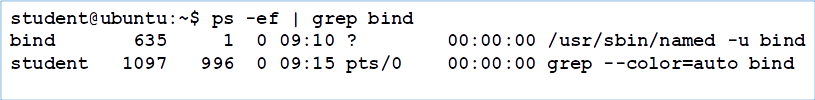
\includegraphics[width=0.9\linewidth]{ps-bind.png}
    \end{center}
  \end{figure}
\end{frame}

\section{Configuration options}
\subsection{Overview}

\begin{frame}{Configuring \texttt{BIND9}}
  \begin{itemize}
    \item Mainly through configuration files.
      \begin{itemize}
        \item located in \texttt{/etc/bind/}
      \end{itemize}
    \item There are several \texttt{DNS} configurations.
      \begin{itemize}
        \item Caching \texttt{DNS}
        \item Primary \texttt{DNS}
        \item Secondary \texttt{DNS}
      \end{itemize}
  \end{itemize}
\end{frame}

\subsection{\texttt{DNS} Architecture}

\begin{frame}{Caching \texttt{DNS}}
  \begin{figure}
    \begin{center}
      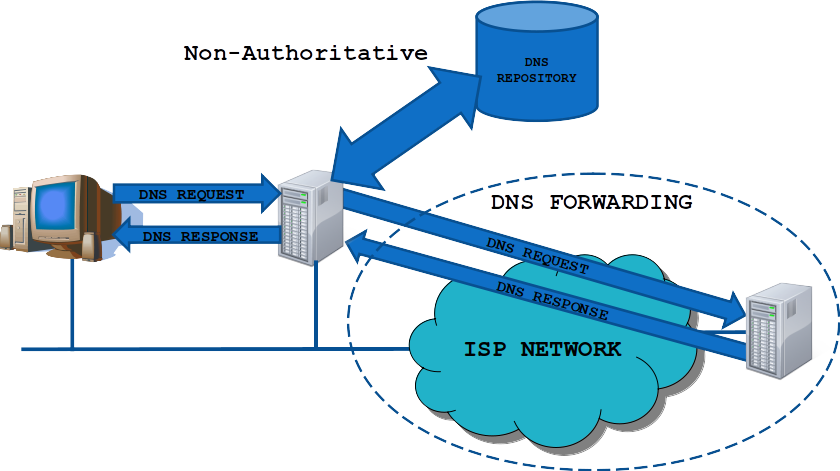
\includegraphics[width=1\linewidth]{cachingdns.png}
    \end{center}
  \end{figure}
\end{frame}

\begin{frame}{Caching \texttt{DNS}}
  \begin{itemize}
    \item Any query that is received will be checked against the internal database.
      \begin{itemize}
        \item If an answer is found then return answer to client.
      \end{itemize}
    \item If not found a forward/recursive lookup will be carried out on another \texttt{DNS} server.
      \begin{itemize}
        \item If an answer is returned from the forwarded \texttt{DNS}.
          \begin{itemize}
            \item store the answer locally.
            \item return answer to client.
          \end{itemize}
        \item If \texttt{not found} answer returned from the forwarded \texttt{DNS}
        \begin{itemize}
          \item store the answer locally (negative cache).
          \item return answer to client.
        \end{itemize}
      \end{itemize}
  \end{itemize} 
\end{frame}

\begin{frame}{Caching \texttt{DNS}}
  \begin{tcolorbox}[title={\textbf{NOTE:}}]
    This module will only be considering \texttt{recursive} and \texttt{forwarded} queries.
  \end{tcolorbox} 
  \end{frame}

\begin{frame}{Primary \texttt{DNS}}
  \begin{figure}
    \begin{center}
      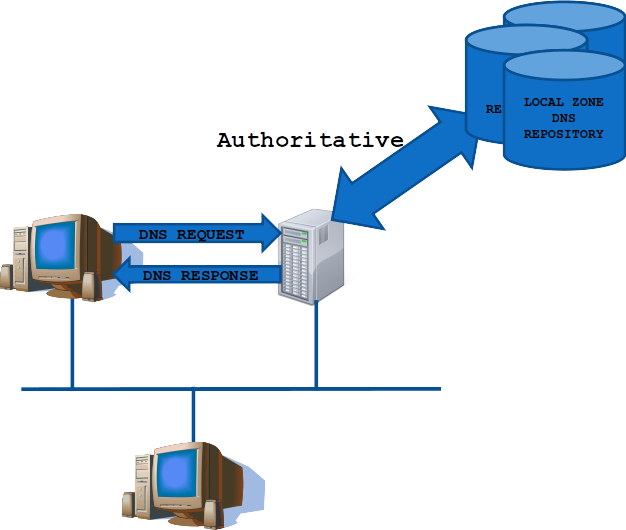
\includegraphics[width=0.75\linewidth]{primarydns.png}
    \end{center}
  \end{figure}
\end{frame}

\begin{frame}{Primary Caching \texttt{DNS}}
  \begin{figure}
    \begin{center}
      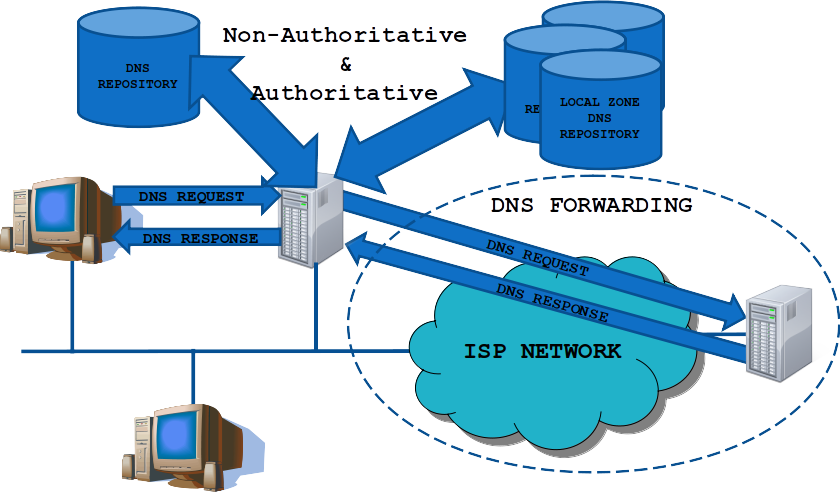
\includegraphics[width=1\linewidth]{primarycachingdns.png}
    \end{center}
  \end{figure}
\end{frame}

\begin{frame}{Secondary \texttt{DNS}}
  \begin{figure}
    \begin{center}
      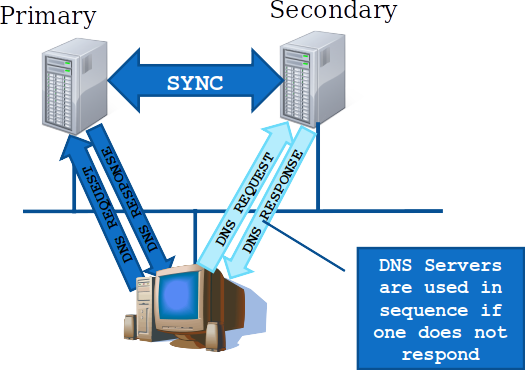
\includegraphics[width=0.9\linewidth]{secondarydns.png}
    \end{center}
  \end{figure}
\end{frame}

\begin{frame}{Primary \texttt{DNS} as master only}
  \begin{figure}
    \begin{center}
      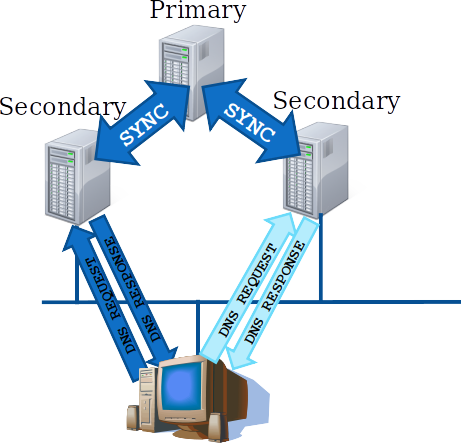
\includegraphics[width=0.65\linewidth]{masteronlydns.png}
    \end{center}
  \end{figure}
\end{frame}

\begin{frame}{Primary \texttt{DNS} as master only}
  \begin{tcolorbox}[title={\textbf{SECURITY:}}]
    \begin{itemize}
      \item Only configure clients to use the \texttt{Secondary servers}.
      \item Configure the \texttt{Primary server} to only allow the \texttt{Secondary servers} to have access.
      \item You could locate the \texttt{Primary server} behind a \texttt{firewall} for added protection.  
    \end{itemize}
  \end{tcolorbox}
\end{frame}

\begin{frame}{\texttt{DNS} Fault Tolerance}
  \begin{figure}
    \begin{center}
      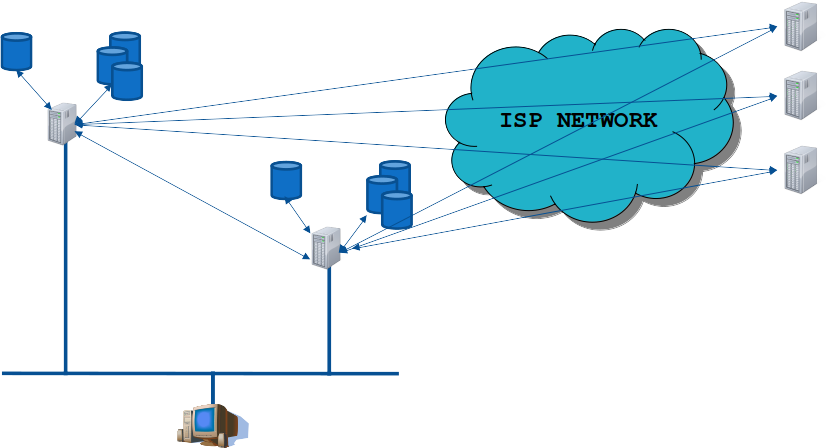
\includegraphics[width=1\linewidth]{faulttolerance.png}
    \end{center}
  \end{figure}
\end{frame}

\section{Configuring \texttt{BIND9}}
\subsection{File Location}
\begin{frame}{Configuring a Caching \texttt{DNS}}
  \begin{itemize}
    \item Main configuration file.
      \begin{itemize}
        \item \texttt{/etc/bind/named.conf.options}
      \end{itemize}
  \end{itemize}
\end{frame}

\subsection{Configuration}
\begin{frame}[fragile]{Default Configuration}
  \begin{lstlisting}
    student@ubuntu:~$ cat /etc/bind/named.conf.options
    options {
            directory "/var/cache/bind";
    
            // If there is a firewall between you and nameservers you want
            // to talk to, you may need to fix the firewall to allow multiple
            // ports to talk.  See http://www.kb.cert.org/vuls/id/800113
    
            // If your ISP provided one or more IP addresses for stable
            // nameservers, you probably want to use them as forwarders.
            // Uncomment the following block, and insert the addresses replacing
            // the all-0's placeholder.
    
            // forwarders {
            //      0.0.0.0;
            // };
            dnssec-validation auto;
            auth-nxdomain no;    # conform to RFC1035
            listen-on-v6 { any; };
    };
  \end{lstlisting}
\end{frame}

\begin{frame}{\texttt{BIND9} Vulnerability}
  \begin{figure}
    \begin{center}
      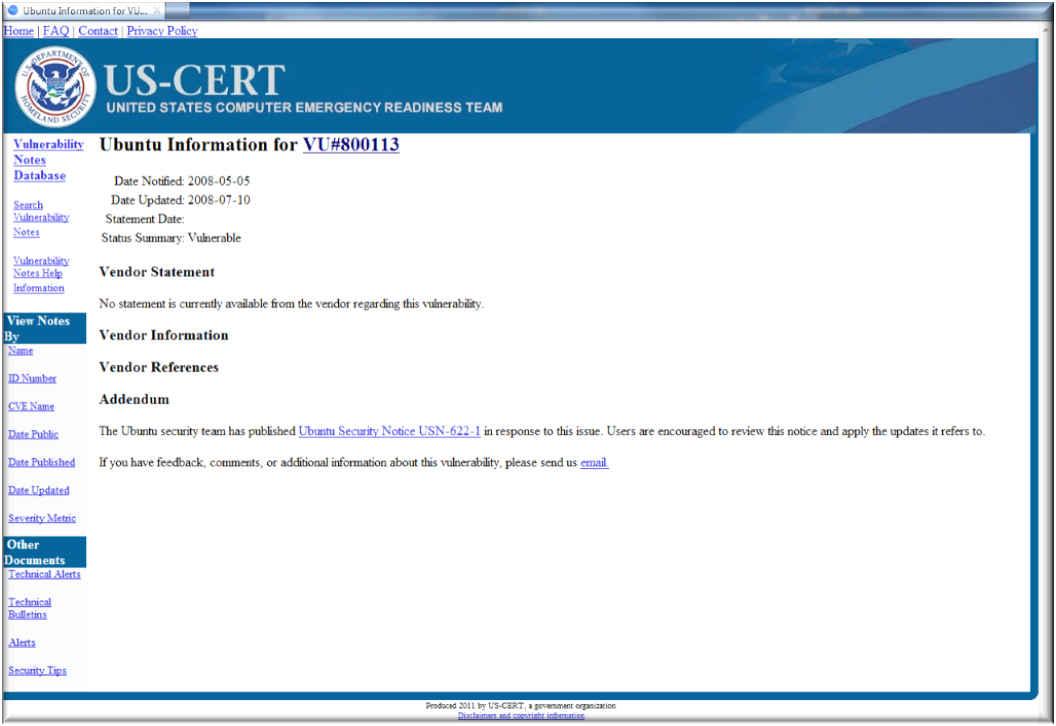
\includegraphics[width=0.9\linewidth]{vulnerability.png}
    \end{center}
  \end{figure}
\end{frame}

\begin{frame}[fragile]{Caching server with \texttt{Forwarders}}
  \begin{lstlisting}
    student@ubuntu:~$ cat /etc/bind/named.conf.options
    options {
        directory "/var/cache/bind";

        // If there is a firewall between you and nameservers you want
        // to talk to, you may need to fix the firewall to allow multiple
        // ports to talk.  See http://www.kb.cert.org/vuls/id/800113

        // If your ISP provided one or more IP addresses for stable
        // nameservers, you probably want to use them as forwarders.
        // Uncomment the following block, and insert the addresses replacing
        // the all-0's placeholder.

        forwarders {
 		      192.168.1.254; 
		      192.168.1.253;
        };
        dnssec-validation auto;
        auth-nxdomain no;    # conform to RFC1035
        listen-on-v6 { any; };
    };
  \end{lstlisting}
  \begin{tcolorbox}[title={\textbf{NOTE:}}]
    \texttt{IP} addresses shown are examples only.
  \end{tcolorbox}
\end{frame}

\subsection{Restarting the daemon}
\begin{frame}{\texttt{systemctl} command}
  \begin{itemize}
    \item \texttt{\$systemctl restart bind9}
  \end{itemize}
  \begin{tcolorbox}[title={\textbf{NOTE:}}]
    There are other commands that can be used but try and stick with the recommended \texttt{systemd} way of doing things.
  \end{tcolorbox} 
\end{frame}

\section*{Conclusion}
\begin{frame}{Conclusion}
  \begin{itemize}
    \item What is the function of a \texttt{DNS} server
    \item What is a \texttt{DNS} architecture?
    \item How does \texttt{Ubuntu Server} support \texttt{DNS}?
    \item How is a simple caching \texttt{DNS} server configured?
  \end{itemize}
\end{frame}

\end{document}


